\chapter{Apéndice A: Estructuras de datos del sistema}
\label{apendiceA}
\lhead{Apéndice A. \emph{Estructuras de datos del sistema}}

% En los apéndices se incluye cualquier información que no sea esencial para la
% comprensión básica del trabajo, pero provea ejemplos y casos de estudio
% extendidos que permitan un análisis más exhaustivo.


\section{Estructura de Datos del Módulo de Segmentación}

En el módulo de segmentación existen tres estructuras de datos fundamentales. Una es utilizada en la función de normalización y la otras dos en
la de segmentación.

\subsection*{Normalización}
\label{ssec:estructuraNormalizacion}

La estructura de datos utilizada en la función de normalización es un hash table que contiene los elementos de un encoding table de tipo UTF-8, en donde las claves de la tabla serían los elementos de tipo UTF-8 y los atributos de las mismas corresponderían a los caracteres sin alguna codificación. Con esta tabla, se quiere implementar un diccionario que mapee los elementos de tipo UTF-8 con sus respectivos caracteres lo mas rapido posible.

Se utilizó un hash table para implementar este diccionario debido a que es ampliamente conocido que este tipo de tablas propocionan mucha eficiencia en el tiempo de búsqueda de sus elementos \cite{Cormen}.

Para implementar este tipo de estructura se utilizó el tipo de dato ``table'' otorgado por el lenguaje de scripting de Bro.

\subsection*{Función de segmentación}
\label{ssec:estructuraSegmentacion}

Por otra parte, la estructura de datos utilizada en la función de segmentación de este módulo es un registro en el cual se almacenan todos los segmentos que se originan a partir de la segmentación de un URI, el URI sin segmentar, un booleano que informa si el URI segmentado sigue con la sintaxis establecida en el RFC 3896, y el número de estados que fueron visitados en el autómata presentado en el modelo teórico.
 
Se escogió un registro para almacenar la información ya que el lenguaje de ``scripting'' de Bro solo presenta como alternativa el tipo de dato ``record'' para crear un tipo de dato compuesto. 

El registro creado esta conformado por los siguientes campos:
\begin{itemize}
\item uri: Es una variable de tipo ``string'' que almacena el URI sin segmentar. Este campo del registro será utilizado por el módulo de entrenamiento al momento de escribir los logs correspondientes.
\item host: Es una variable de tipo ``hash table'' cuyas claves son número y sus valores  son de tipo string. En esta sección se almacenan los segmentos del URI correspondiente al host.
\item path: Es una variable de tipo ``hash table'' cuyas claves son número y sus valores  son de tipo string. En esta sección se almacenan los segmentos del URI correspondiente al path.
\item query: Es una variable de tipo ``hash table'' cuyas claves y sus valores son de tipo string. En esta sección se almacenan los atributos y los valores del query del URI en caso de que el mismo posea. Los atributos y los valores se almacenarán en una hash table como se mencionó con anterioridad, en donde la clave del mismo serán los atributos del query y en donde los valores de las misma serán los valores del query del URI.
\item fragment: Es una variable de tipo ``string'' que almacenará el fragment del URI en caso de poseerlo.
\item número de estados: es una variable de tipo entero que almacena el número de estados del autómata que se emplea en el módelo teórico fueron visitados para reconocer el URI. Este campo del registro será utilizado por el módulo de evaluación.
\item uri correcto: es una variable de tipo booleano que indica si el URI está sintácticamente correcto o no.
\end{itemize}

El nombre que recibirá este tipo de estructura es ``UriSegmentado''. La misma se puede apreciar gráficamente en la figura \ref{fig:uriSegmentado}.

\begin{figure}[!htb]
\begin{center}
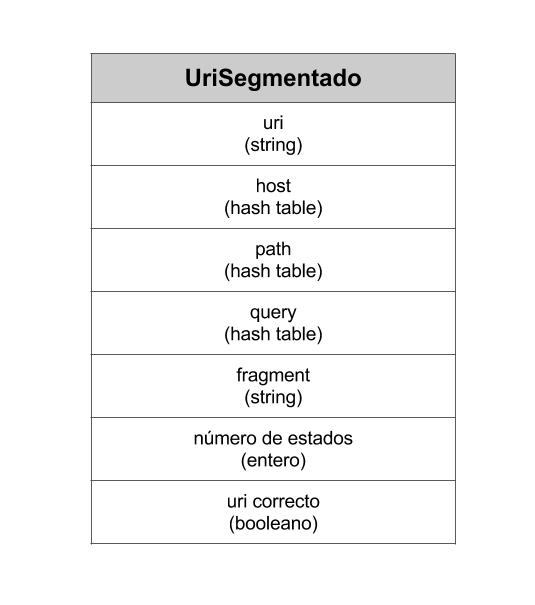
\includegraphics[width=4in]{./img/UriSegmentado.jpg}
\caption{Ejemplo gráfico de la estructura ``UriSegmentado''.}
\label{fig:uriSegmentado}
\end{center}
\end{figure}

Además de utilizar el tipo de dato ``UriSegmentado'', el módulo de segmentación hace uso de una estructura de datos compuesta, primitiva del lenguaje de ``scripting'' de Bro llamada  ``URI''. Dicha estructura posee los siguientes campos:

\begin{itemize}
\item scheme: Es un campo opcional de tipo ``string'' que almacena el protocolo del URI.

\item netlocation: Es un campo de tipo ``string'' que almacena el nombre de dominio o la dirección IP del URI.

\item portnum: Es un campo opcional de tipo ``count''  que almacena el número de puerto del URI.
\item path:Es un campo de tipo ``string'' que almacena la ruta del URI.

\item file\_name: En un campo opcional de tipo ``string'' que almacena el nombre completo  del archivo de la ruta del URI junto a su extensión.

\item file\_base: En un campo opcional de tipo ``string'' que almacena el nombre  del archivo de la ruta del URI sin su extensión.

\item file\_ext: En un campo opcional de tipo ``string'' que almacena la extensión del archivo de la ruta.

\item params: Es un campo opcional de tipo ``table'' que almacena todos los parámetros de la consulta del URI. Esta tabla mapea todos los atributos con sus valores.

\end{itemize}

La estructura ``URI'' se puede apreciar gráficamente en la figura \ref{fig:URI}.

\begin{figure}[!htb]
\begin{center}
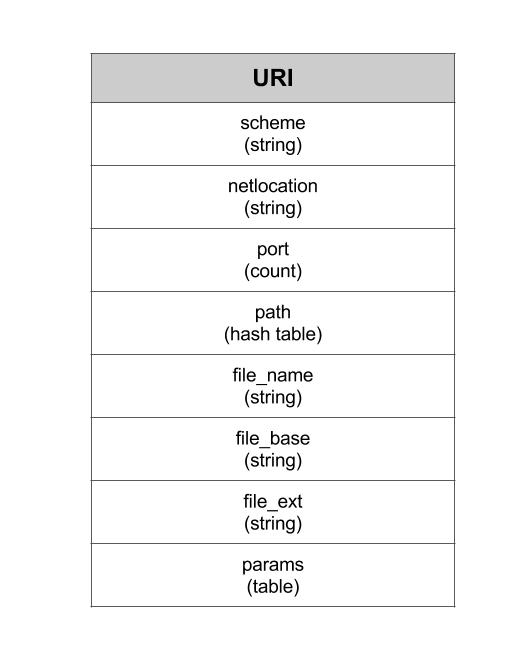
\includegraphics[width=4in]{./img/URIstruct.jpg}
\caption{Ejemplo gráfico de la estructura ``URI''.}
\label{fig:URI}
\end{center}
\end{figure}	



\section{Estructura de Datos del Módulo de Evaluación}

El módulo de evaluación del sistema cuenta con varias estructura de datos compuestas de tipo ``register'' y de tipo ``table'' que serán explicados a continuación 

\subsection*{Modelo de normalidad}
\label{sssec:estructuraModelo}

Existen dos estructuras de tipo ``register'' en la función para leer el modelo de normalidad y dos de tipo ``table''.
Las estructuras de tipo ``register'' poseen los siguientes campo:

La primera, cuyo nombre es ``Word'' posee los siguientes campo:
\begin{itemize}
\item ``word'' es un campo de tipo ``string'' en donde se almacenarán las palabras del vocabulario de cada uno de los estados del autómata presentado en la imagen \ref{fig:ssm}.
\item ``state'' es un campo de tipo string en donde se indicará el estado del autómata presentado en la imagen \ref{fig:ssm} al que pertenece la palabra almacenada en el campo ``word''.
\end{itemize}

Esta estructura se puede observar de manera gráfica en la figura \ref{fig:WORD}.

\begin{figure}[!htb]
\begin{center}
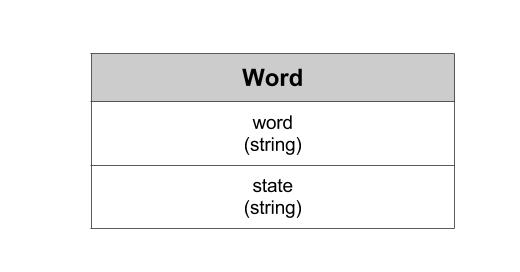
\includegraphics[width=4in]{./img/Word.jpg}
\caption{Ejemplo gráfico de la estructura ``Word''.}
\label{fig:WORD}
\end{center}
\end{figure}	

La segunda estructura llamada ``Probability'' solo posee un campo llamado ``probability''.
\begin{itemize}
\item ``probability'' es un campo de tipo ``double'' en donde se almacenará la probabilidad de generación de las palabras que se encuentran en el modelo.
\end{itemize}

Se puede observar un ejemplo gráfico de la estructura en la figura \ref{fig:Probability}.

\begin{figure}[!htb]
\begin{center}
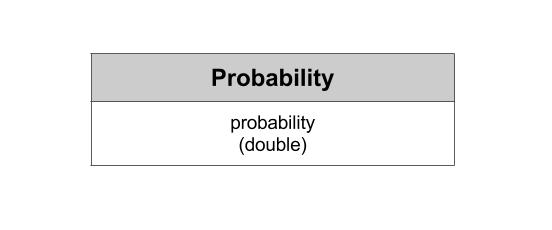
\includegraphics[width=4in]{./img/Probability.jpg}
\caption{Ejemplo gráfico de la estructura ``Probability''.}
\label{fig:Probability}
\end{center}
\end{figure}	

La tercera estructura de tipo ``register'' que será utilizada en el módulo de evaluación se llamada ``TableDescription'' y pertenece al módulo ``Input'' de Bro y se utilizará al momento de leer los archivos de entrada.
Los campos utilizados de esta estructura fueron los siguientes:
\begin{itemize}
\item source: campo de tipo ``string'' que almacena el nombre del archivo
que va a ser leído.
\item name: campo de tipo ``string'' que almacenará el nombre que se le
asignará al flujo de entrada.
\item destination: Nombre de la tabla que almacena la información contenida
en los archivos.
\item idx: Nombre del registro que definirá los valores que utilizará la tabla que almacena la información del archivo como clave.
\item val: Campo opcional que almacena el nombre del registro que define
los valores de la tabla que almacena la información de los archivos de
entrada.
\end{itemize}

En la figura \ref{fig:TableDescription} se muestra un ejemplo gráfico de ``TableDescription''.

\begin{figure}[!htb]
\begin{center}
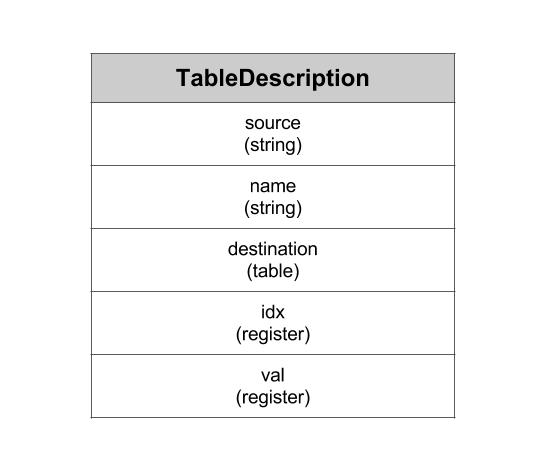
\includegraphics[width=4in]{./img/TableDescription.jpg}
\caption{Ejemplo gráfico de la estructura ``TableDescription''.}
\label{fig:TableDescription}
\end{center}
\end{figure}	

Por otra parte, las estructuras de tipo ``table'' son dos. Una tabla será utilizada para almacenar las palabras del vocabulario, la probabilidad de generación y el nombre del estado al que pertenece dicha información mientras que la otra almacenará las probabilidades de fuera de vocabulario de cada uno de los estados y el valor del parámetro $\theta$ presente en la expresión \ref{eq:ClaseU}.

La primera tabla es una ``hash table'' que posee dos elementos tipo ``string'' como clave, y como valor tiene un campo de tipo ``Probability''.

Esta tabla almacenará el modelo de normalidad del sistema, es decir, las palabras del vocabulario, la probabilidad de generación de las mismas y el estado al que pertenece dicha información. Las claves de esta tabla serán las palabras del vocabulario y el nombre del estado al que pertenecen. Toda esta informacion será dada a través de un archivo de texto cuya estructura será explicada en las sección ~\ref{sec:lecturaModelo}.

La segunda tabla es una hash table que tendrá solo un elemento como clave de tipo ``string''. Los valores de la misma serán campo tipo ``Valor''. 

En dicha tabla se van a almacenar las probabilidades de fuera de vocabulario de cada uno de los estados del autómata y el parámetro $\theta$. La clave de la misma sería una cadena de caracteres que identifique cada una de las probabilidades  y el parámetro  $\theta$. Esas etiquetas serían las siguientes: Poov1, Poov2, Poov3, Poov4, Theta.  

\subsection*{Evaluación de las probabilidades de los URI}
\label{sssec:estructuraEvaluacion}

La función  que se encarga de calcular el índice de anormalidad  y evaluar si el mismo es anómalo o no, solo contiene una estructura compuesta de tipo ``record'' y se utiliza junto a una herramienta de Bro que funciona para escribir ``logs''. Los ``logs'' que son escritos a través de esta herramienta son archivos de texto que contiene una lista de los URI que presentan anomalías.

La estructura lleva como nombre ``InfoAtaque'' y contiene los siguientes campos:

\begin{itemize}
\item clasificacion: es un campo de tipo ``string'' que almacena la clasificación de los URIs anómalos, es decir, aquí se indica si el mismo presenta anomalía por estar sintácticamente mal construidos o porque el índice de anormalidad sobrepasó el parámetro $\theta$.
\item uri: es un campo de tipo ``string'' en el que se va a almacenar el uri que va a ser registrado en el log.
\item probability: es un campo de tipo ``string'' en donde se va a almacenar el valor del índice de anormalidad del uri.
\end{itemize}

Todos los campos anteriormente descritos poseen la cualidad de ser de tipo ``log'' tambien. Con esto se indica cuál de los elementos de la estructura de datos se escribirá sobre los logs.

    El registro ``InfoAtaque'' se puede observar de manera gráfica en la figura \ref{fig:InfoAtaque}. 
    
\begin{figure}[!htb]
\begin{center}
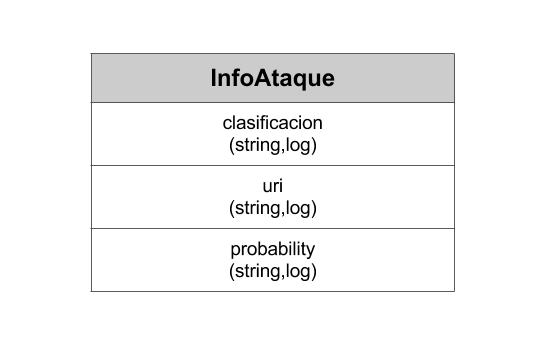
\includegraphics[width=4in]{./img/InfoAtaque.jpg}
\caption{Ejemplo gráfico de la estructura ``InfoAtaque''.}
\label{fig:InfoAtaque}
\end{center}
\end{figure}	



\section{Estructura de Datos del Módulo de Entrenamiento}
El módulo de entrenamiento consta de varias estructuras de datos de
tipo ``register'' y de tipo ``table'' para realizar su trabajo. Tanto el modo
``Online'' como el ``Offline'' comparten las mismas estructuras.
La estructuras serían las siguientes:
``Entrenamiento'' es una estructura de tipo ``record'', cuyo funcionamiento es ir almacenando el número de veces que una palabra es observada junto con la probabilidad de observación, mientras se realiza el entrenamiento. Los
campos de esta estructura son los siguientes:

\begin{itemize}
\item numPalabras: campo de tipo entero que almacena el número de veces
que una palabra es observada durante el entrenamiento.
\item probability: campo de tipo flotante que almacene la probabilidad de observación de una palabra.
\end{itemize}

Un ejemplo gráfico de la estructura ``Entrenamiento'' se puede apreciar
en la figura \ref{fig:figEntrenamiento}.
La otra estructura de tipo ``record'' es ``Info''. ``Info'' se encargará de
almacenar la información que será escrita en el archivo de texto que representará el modelo de normalidad. Los campos de esta estructura de datos
son los siguientes:

\begin{figure}[!htb]
\begin{center}
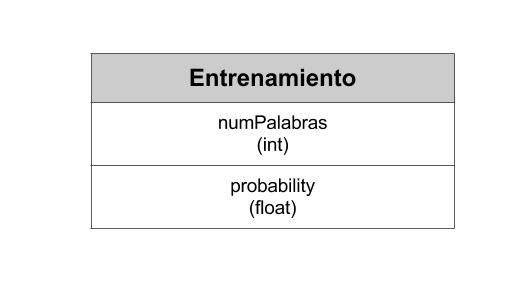
\includegraphics[width=4in]{./img/EntrenamientoRegister.jpg}
\caption{Ejemplo gráfico de la estructura ``Entrenamiento''.}
\label{fig:figEntrenamiento}
\end{center}
\end{figure}	

\begin{itemize}
\item state: es un campo de tipo ``string'' que almacenará el nombre del
estado al que pertenece la palabra y su probabilidad de observación.
\item word: es un campo de tipo ``string'' que almacenará las palabras observadas durante el entrenamiento.
\item probability: es un campo de tipo flotante que almacenará la probabilidad de observación de las palabras.
\end{itemize}

La estructura ``Info'' se puede observar de manera gráfica en la figura
\ref{fig:figInfo}.

\begin{figure}[!htb]
\begin{center}
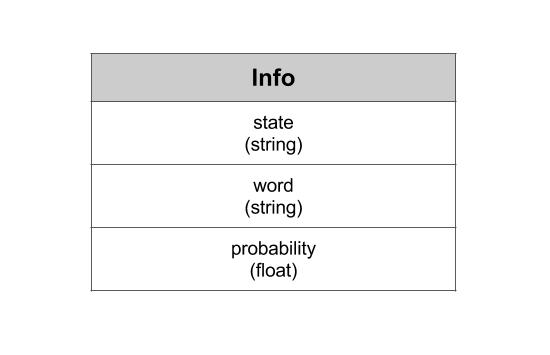
\includegraphics[width=4in]{./img/Info.jpg}
\caption{Ejemplo gráfico de la estructura ``Entrenamiento''.}
\label{fig:figInfo}
\end{center}
\end{figure}

Por otra parte, la estructura tipo ``table'' que se utilizó en la implementación de este módulo fueron las siguientes:
Se hizo uso de una tabla de hash que posee como clave un campo tipo
``string'' y como valor una estructura de datos de tipo ``Entrenamiento''
(fig. \ref{fig:figEntrenamiento}). Esta tabla tendrá como función almacenar las palabras que van apareciendo durante el entrenamiento, el número de veces que fueron observadas las mismas y la probabilidad de aparición . La clave de esta tabla serán las palabras observadas y el resto de la informacion sería almacenado en la estructura de datos ``Entrenamiento''.
Cada estado del autómata tendrá su tabla de entrenamiento propia para
de esta manera tener una mayor organización de las observaciones realizadas durante el entrenamiento.
